
\section{{Part I}}

%	{In this particular lab experiment, the component of physics known as circular motion was introduced. This area of physics analyzes the fundamental behavior and laws that an object adhere's to when the object moves around a circular path. An important part of this is circular acceleration, or as it’s known as centripetal acceleration. Therfore we have,}

	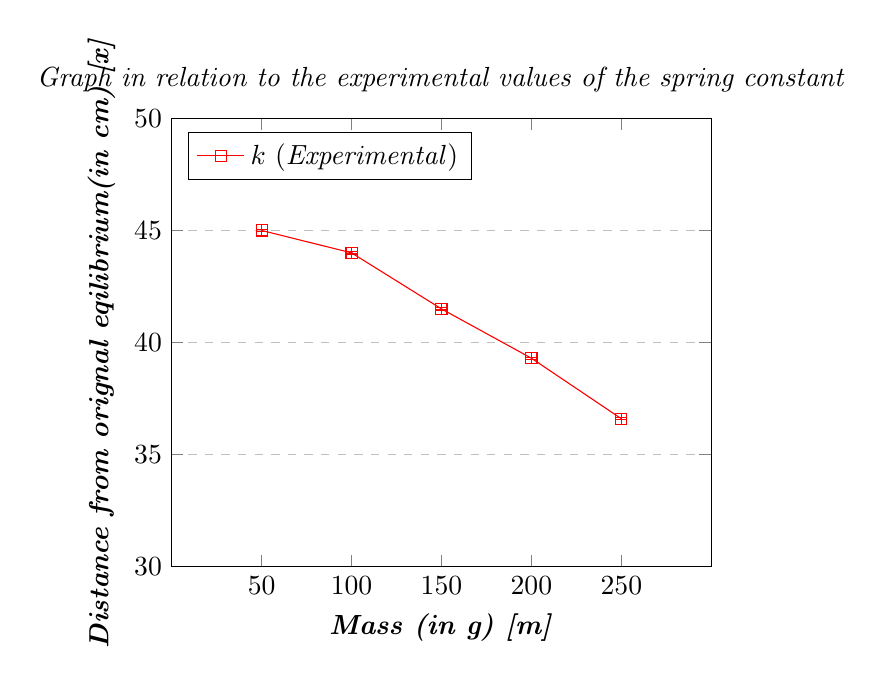
\begin{tikzpicture}
            \begin{axis}[
                title={\textit{Graph in relation to the experimental values of the spring constant}},
                xlabel={\textbf{\textit{Mass (in g) [m]}}},
                ylabel={\textbf{\textit{Distance from orignal eqilibrium(in cm) [x]}}},
                xmin=0, xmax=300,
                ymin=30, ymax=50,
                xtick={50,100,150,200,250},
                ytick={30,35,40,45,50},
                legend pos=north west,
                ymajorgrids=true,
                grid style=dashed,
                legend entries={$k$ (\textit{Experimental})}
            ]
            
            \addplot+[
                color=red,
                mark=square,
                ] plot[error bars/.cd, y dir=both, y explicit, x dir=both, x explicit]
                coordinates {
                (50,45) +- (0.01,0.05)
                (100,44) +- (0.01,0.05)
                (150,41.5) +- (0.01,0.05)
                (200,39.3) +- (0.01,0.05)
                (250,36.6) +- (0.01,0.05)
                };
                
            \end{axis}
        \end{tikzpicture}

	{We know that when the mass is attached to the spring, results in the spring being streched from its equilibrium position, resulting in an new equilibrium position. This is due to the force acting on the spring-mass system due to gravity. Therfore we have, }

		$$F_{g} = mg$$

	{We also know that the Spring force is mathematically represented as,}

		$$F_{s} = -kx$$

	{As we know that the spring eventually comes to an equilibrium length, where the forces equal, we have,}
	
		$$F_{s} = F_{g}$$	
	
	{Therfore,}	
	
		$$mg = -kx \implies k = -\frac{m}{x}g$$	
	
	{Therefore from the above graph, we have,}	
	
		$$k \approx 1.246 \text{ N/m}$$	
	
\section{{Part II}}	
	
	{We know that,}
		
		$$x\left(t\right) = A\cos\left(\omega t + \phi\right)$$
		
	{We also know that,}		
		
		$$\omega = \frac{2\pi}{T} = \frac{2\pi}{0.8} = 7.85 \text{ rad/s}$$
	
	{Therfore,}
	
		$$y\left(t\right) = A\cos\left(7.85t + \phi\right)$$
		
	{Also,}
	
		$$y\left(0\right) = A\cos\left(\phi\right)$$
		
	{Therfore,}		
		
		$$\phi = \text{ 1.87 rad}$$
	
	\textbf{This implies that the phase of the system which is $\phi$ is 1.87 rad.}	
	
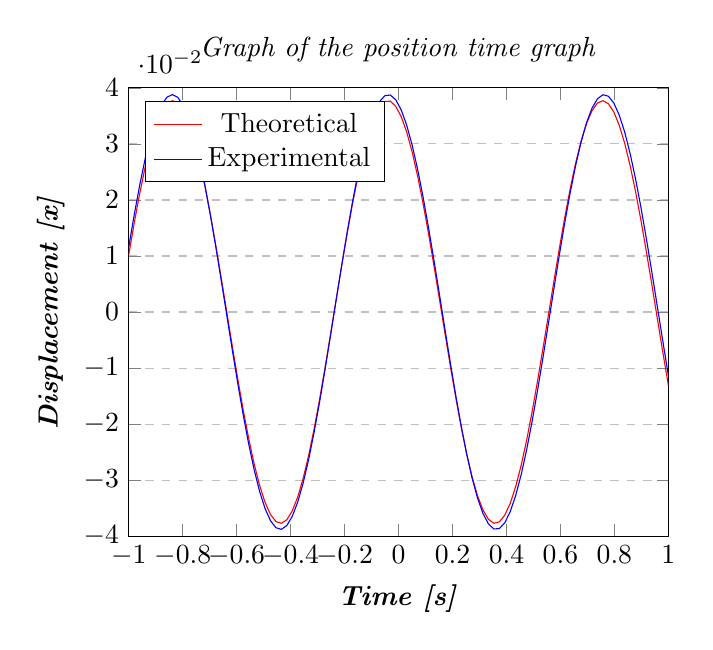
\begin{tikzpicture}
\begin{axis}[
                title={\textit{Graph of the position time graph}},
                xlabel={\textbf{\textit{Time [s]}}},
                ylabel={\textbf{\textit{Displacement [x]}}},
                xmin=-1, xmax=1,
                ymin=-0.04, ymax=0.04,
                xtick={-1,-0.8,-0.6,-0.4,-0.2,0,0.2,0.4,0.6,0.8,1},
                ytick={-0.04,-0.03,-0.02,-0.01,0,0.01,0.02,0.03,0.04},
                legend pos=north west,
                ymajorgrids=true,
                grid style=dashed,
                legend entries={$\frac{20\cdot\mu_0}{\pi}$ (\textit{Experimental})}
            ]
%Below the red parabola is defined
\addplot [
    domain=-1:1, 
    samples=100, 
    color=red,
]
{0.03772 * sin(deg(7.894 * x + 1.884))};
\addlegendentry{Theoretical}
%Here the blue parabola is defined
\addplot [
    domain=-1:1, 
    samples=100, 
    color=blue,
    ]
    {0.0388 * sin(deg(7.85 * x + 1.87))};
\addlegendentry{Experimental}

\end{axis}
\end{tikzpicture}	

	{After using the Sine curve of the form, $A\sin\left(Bx + C\right)$ to fit the data from the above graph, the values for A, B \& C are,}
			
	\begin{table}[H]
    \centering
    		\begin{tabular}{|c|c|}
    			\hline
    			\hline
        		Expected Value & Measured Value \\
        		\hline
        		$A = 0.03772$ m & $A = 0.03885$ m \\
        		\hline
        		$B = 7.894$ rad/s & $B = 7.85$ rad/s \\
        		\hline
        		$C = 1.884$ rads & $C = 1.87$ rads \\
			\hline        		
        		\hline
    		\end{tabular}
    		\caption{Values of A, B \& C in the form $A\sin\left(Bx + C\right)$ that describes the motion of the system}
    		\label{Part II}
	\end{table}

	{We now know that, $\omega = B$, therefore $\omega = 7.85\text{ rad/s}$}

	{Therefore,}

		$$\omega = 7.85 = \sqrt{\frac{k}{m}}$$

		$$\implies k = 18.49 \text{ N/m}$$